% -*- root: ../Presentation.tex -*-
\section{Steganalysis}
\begin{frame}{Steganalysis}{}
	Steganalysis techniques used:
	\begin{itemize}
		\item Colour histogram
		\item LSB enhancing
		\item Comparing image with original image
		\item DCT coefficients histogram
		\item Steganographic signatures/patterns
	\end{itemize}
\end{frame}

\subsection{Colour histogram}
\begin{frame}{Colour histogram}{}
\begin{figure}
\centering     %%% not \center
\subfigure[]{\label{fig:a}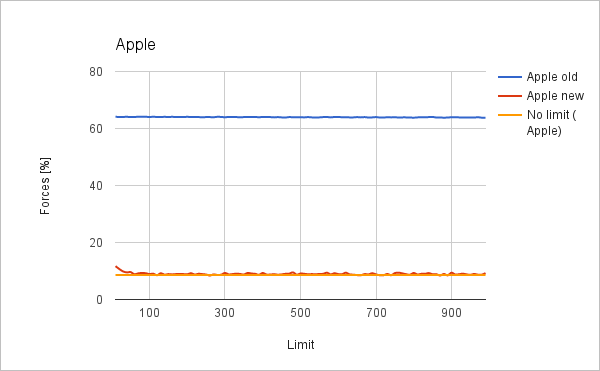
\includegraphics[width=.4\textwidth]{figures/graphApple.png}}
\subfigure[]{\label{fig:b}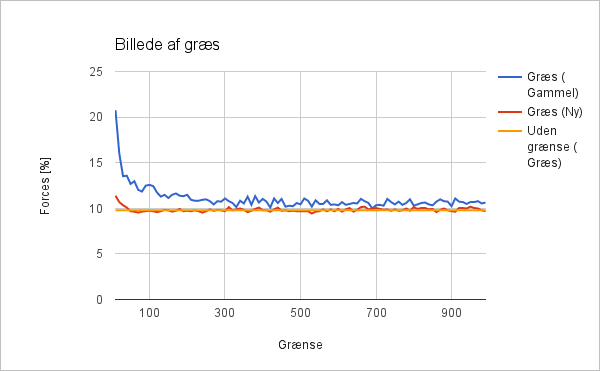
\includegraphics[width=.4\textwidth]{figures/graphGrass.png}}
\subfigure[]{\label{fig:a}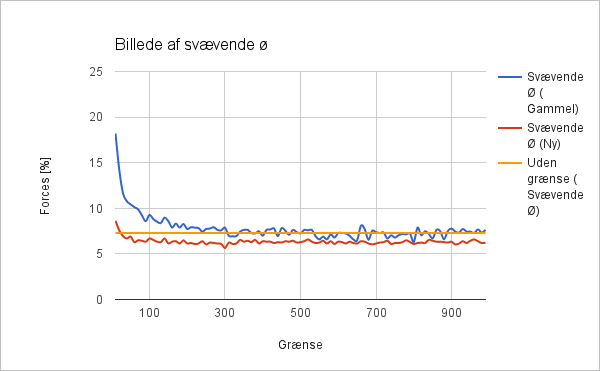
\includegraphics[width=.4\textwidth]{figures/graphIsland.png}}
\caption{Sammenligning af colour histogram}
\label{fig:limits}
\end{figure}
\end{frame}

\subsection{LSB enhancing}
\begin{frame}{LSB enhancing}
\end{frame}

\subsection{Comparing image with original image}
\begin{frame}{looking at how images differ from original}
\begin{figure}
\centering
\subfigure[]{\label{fig:a}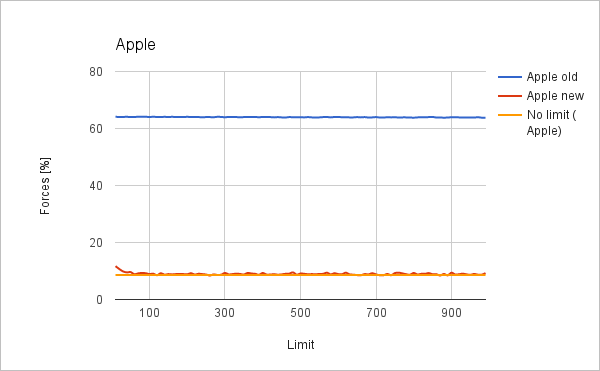
\includegraphics[width=.4\textwidth]{figures/graphApple.png}}
\subfigure[]{\label{fig:b}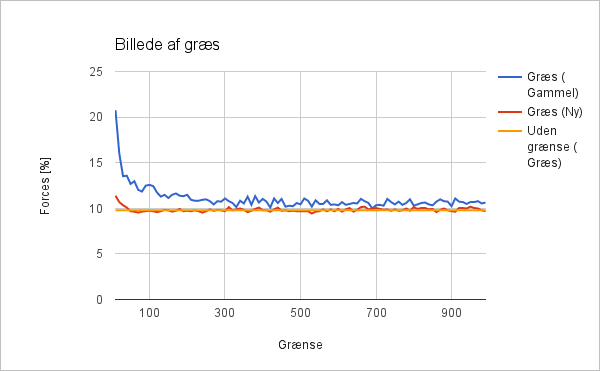
\includegraphics[width=.4\textwidth]{figures/graphGrass.png}}
\subfigure[]{\label{fig:a}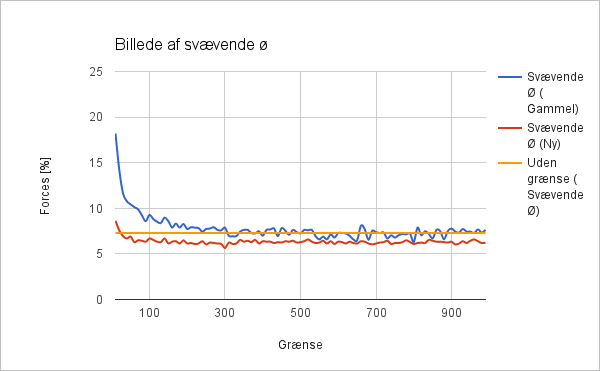
\includegraphics[width=.4\textwidth]{figures/graphIsland.png}}
\caption{Sammenlligning af bileder}
\end{figure}
\end{frame}